\documentclass[11pt]{article}
\setlength{\oddsidemargin}{0in}
\setlength{\evensidemargin}{0in}
\setlength{\textwidth}{6.5in}

\usepackage{fancyhdr}
\pagestyle{fancy}
\usepackage{amsmath,amsfonts,amssymb}
\usepackage{epsfig}
\usepackage{subfigure}
\usepackage{placeins}
\usepackage{amsmath}
\usepackage[usenames,dvipsnames,svgnames,table]{xcolor}
\usepackage{amssymb}
\usepackage{setspace}
\usepackage{graphicx} % Include figure files
\usepackage{times}
\usepackage{amsthm}
\usepackage{hyperref}
\usepackage{enumitem}
\hypersetup{bookmarks=true, unicode=false, pdftoolbar=true, pdfmenubar=true, pdffitwindow=false, pdfstartview={FitH}, pdfcreator={Daniel Larremore}, pdfproducer={Daniel Larremore}, pdfkeywords={} {} {}, pdfnewwindow=true, colorlinks=true, linkcolor=blue, citecolor=Green, filecolor=magenta, urlcolor=cyan,}
\usepackage[parfill]{parskip}
\usepackage{tikz}
\usetikzlibrary{arrows.meta, positioning}

\graphicspath{{plots}{./}}

\newcommand{\e}{\mathrm{e}}
\renewcommand{\d}{\mathrm{d}}
\newcommand{\erf}{\mathop\mathrm{erf}}
\newcommand{\erfc}{\mathop\mathrm{erfc}}
\newcommand{\xmin}{\ensuremath{x_{\min}}}
\newcommand{\ntail}{\ensuremath{n_{\rm tail}}}

\newcommand{\Q}[1]{\footnote{\textcolor{blue}{#1}}}

\begin{document}

\lhead{{\bf Mathematical \& Computational Modeling of Infectious Diseases \\ 
Homework 2}}
\rhead{{\bf D.B.\ Larremore\\2025}}
\renewcommand{\headrulewidth}{0.4pt}

{\bf Name:} Ben Aoki-Sherwood

{\bf Collaborators: } Altaf Barelvi and Violet Ross

{\bf Code: } \url{https://github.com/aoki-sherwoodb/CSCI-5897-InfectiousDiseases/blob/main/hw2/hw2.ipynb}
\vspace{0.1in}\hrule

\begin{enumerate}
	\item The goal of this problem is to develop flexibility with your Forward Euler code, and to learn a bit about the effect of step size on the accuracy of the solution.
	
\begin{enumerate}[label=\alph*.]
	\item Using your Forward Euler method, simulate the solution to the {\it normalized} SIS model discussed in class (Week 3) using $\beta=3$ and $\gamma=2$, and with $(s_0, i_0) = (0.99, 0.01)$. Create three plots ranging from $t=0$ to $t=25$. On the first, simulate using a step size $\Delta t=2$. On the second, use $\Delta t =1$. On the third, use $\Delta t = \tfrac{1}{2}$. In each plot, show only your solution's $I(t)$ in a red solid line, labeled as ``Forward Euler'', and then also plot the analytical solution from class in a black dashed line, labeled as ``Analytical.'' Please also set the y-axis range to $[0,0.5]$. 
	
	\begin{figure*}[h]
	\centering
	\includegraphics[width=\textwidth]{sis_forward_euler.png}
	\caption{Normalized SIS model simulated using Forward Euler with time steps of 2, 1, and 0.5. 
	The simulated infected fraction is plotted in red and the analytical solution for the infected compartment is plotted in black.}
	\end{figure*}

	\item Comment on what you see in your three plots. How does the step size affect our solution?
	
	{\bf
	The error of the simulated solution decreases as the step size decreases. 
	The simulated solution systematically underestimates the analytical value during the exponential growth phase because the derivative is increasing, so FE is using an estimate of the derivative that is smaller than the actual derivative.
	Backward Euler would overestimate the solution during this phase.
	When $\Delta t = 2$, the simulated solution oscillates around the analytical equilibrium instead of converging to the equilibrium.
	However, for the smaller step sizes, the simulated solution does converge to the equilibrium.
	}
	\item Define the maximum absolute error for a simulation using a particular $\Delta t$ as $$E(\Delta t) = \max_{t} \big | I_{\text{Euler}, \Delta t} (t) - I_\text{analytical}(t) \big |\ .$$ Write a function that runs the appropriate simulation, computes the analytical solution, and returns $E$ without plotting. Share a link to your code for this problem.
	
	{\bf
	See the code cell under markdown header 1c: \url{https://github.com/aoki-sherwoodb/CSCI-5897-InfectiousDiseases/blob/main/hw2/hw2.ipynb}
	}
	
	\item Create a plot on log-log axes showing $E(\Delta t)$ vs $\Delta t$ for values $$\Delta t \in \{2,1,\tfrac{1}{2},\tfrac{1}{4},\tfrac{1}{8},\tfrac{1}{16},\tfrac{1}{32}\}$$
	
	\begin{figure*}[h]
	\centering
	\includegraphics[width=0.7\textwidth]{plots/max_abs_err_vs_dt.png}
	\caption{Maximum absolute error $E(\Delta t)$ vs step size $\Delta t$ on log-log axes.}
	\end{figure*}

	\item Comment on what you observe in this plot, and comment on cases when you would want a larger or smaller step size, and why? Imagining yourself in an advisory position in your community, can you think of any scenario where there is a connection between the step size of your simulation and the ethics of your advice?

	{\bf This plot shows that error increases roughly linearly with step size.
	In all cases, we want to use as small a step size as is computationally feasible to minimize error. 
	A good check is to halve the step size and see if the solution changes significantly; if not, then the step size is small enough.
	The only case where we might have to use a larger step size is if the model is extremely complex so that simulating many steps takes a long time.
	In an advisory position, we would always want to ensure that our advice is based on \emph{real} (model) dynamics rather than \emph{solver-induced} dynamics.
	We could do this by checking the step size as described above or trying a different solver algorithm.}
\end{enumerate}

\clearpage
	\item The goal of this problem is to get you thinking about the constraints on population contact structure and contact matrices, as well as sensitivity analyses.
	
\begin{enumerate}[label=\alph*.]
	\item As one who is interested in modeling disease transmission on college campuses, you hire two teams to measure contact patterns on a nearby campus. The first team, led by Dan Pemic, tells you that there are $200$ faculty and $1800$ students, with a contact matrix of 
	$$C_\text{Pemic} = \begin{pmatrix}
		3.1 & 43.5 \\
		4.7 & 25.0
	\end{pmatrix}$$
The second team, led by Flynn Uenza, tells you that there are $210$ faculty and $1750$ students, with a contact matrix of
	$$C_\text{Uenza} = \begin{pmatrix}
		3.0 & 44.5 \\
		4.8 & 25.1
		\end{pmatrix}
	$$
Whom do you trust more, Dan Pemic or Flynn Uenza? To answer this question, consider the self-consistency (or lack thereof) of each dataset. Explain your reasoning in words and include any calculations used to arrive at your conclusions. 

{\bf 
Dan Pemic's data is more self-consistent. 
We can calculate the total number student-faculty and faculty-student contacts by multiplying the off-diagonal entries in the contact matrix by the appropriate population sizes.
These numbers should be equal because contacts are symmetric.
For Dan Pemic's data, this yields $$4.7 \cdot 1800 = 8460, 43.5 \cdot 200 = 8700,$$
while for Flynn Uenza's data this yields $$4.8 \cdot 1750 = 8400, 44.5 \cdot 210 = 9345.$$
The discrepancy between student-faculty and faculty-student contacts is smaller for Dan Pemic. 
}
\item A straightforward fix to self-consistency issues is to ``symmetrize'' the rates. First, we compute the implied total number of intergroup contacts from faculty to students, and then compute the same from students to faculty. After averaging those two counts, divide by the appropriate population size to get per-person rates. Use this approach to symmetrize the two contact matrices. 

{\bf
From part a., we have the total number of intergroup contacts for each dataset.
The average number of intergroup contacts from Pemic is $\frac{8460 + 8700}{2} = 8580$, and from Uenza is $\frac{8400 + 9345}{2} = 8872.5$.
Dividing by the number of students for the lower left entry and the number of faculty for the upper right entry yields the contact matrices
$$C_{\text{Pemic}} = \begin{bmatrix}
	3.1 & 42.9 \\
	4.77 & 25.0
\end{bmatrix}$$
and
$$C_{\text{Uenza}} = \begin{bmatrix}
	3.0 & 42.25 \\
	5.07 & 25.1
\end{bmatrix}$$
}

\item How different are these two symmetrized matrices, really? Answer the question by computing the ratio of $R_0$ under Pemic's data to $R_0$ under Uenza's data, assuming SIR models with otherwise identical parameters.

{\bf
We compute $R_0$ as the largest eigenvalue of the next-generation matrix evaluated at the disease-free equilibrium.
Assigning faculty subscript 1 and students subscript 2, this matrix is given by 
$$G_0 = \begin{bmatrix}
	\frac{N_1 p c_{11}}{N_1\gamma} & \frac{N_1 p c_{12}}{N_2 \gamma} \\
	\frac{N_2 p c_{21}}{N_1 \gamma} & \frac{N_2 p c_{22}}{N_2 \gamma}
\end{bmatrix}$$

and we compute its largest eigenvalue using the quadratic formula as 
$$R_0 = \frac{\text{Tr}(G_0) + \sqrt{\text{Tr}(G_0)^2 - 4\text{det}(G_0)}}{2}$$
where $\text{Tr}(G_0) = \frac{p}{\gamma}(c_{11} + c_{22})$ is the trace and $\text{det}(G_0) = \frac{p^2}{\gamma^2}(c_{11}c_{22} - c_{12}c_{21})$ is the determinant.

Thus the ratio of $R_0$ under Pemic's data to $R_0$ under Uenza's data is
}
\begin{align*}
\frac{R_{0,\text{Pemic}}}{R_{0,\text{Uenza}}} &= \frac{-\text{Tr}(G_{0,\text{Pemic}}) + \sqrt{\text{Tr}(G_{0,\text{Pemic}})^2 - 4\text{det}(G_{0,\text{Pemic}})}}{-\text{Tr}(G_{0,\text{Uenza}}) + \sqrt{\text{Tr}(G_{0,\text{Uenza}})^2 - 4\text{det}(G_{0,\text{Uenza}})}} \\
&= \frac{\frac{p}{\gamma}(3.1 + 25.0) + \sqrt{\left(\frac{p}{\gamma}(3.1 + 25.0)\right)^2 - 4\frac{p^2}{\gamma^2}(3.1 \cdot 25.0 - 42.9 \cdot 4.77)}}{\frac{p}{\gamma}(3.0 + 25.1) + \sqrt{\left(\frac{p}{\gamma}(3.0 + 25.1)\right)^2 - 4\frac{p^2}{\gamma^2}(3.0 \cdot 25.1 - 42.25 \cdot 5.07)}} \\
&= \frac{28.1 + \sqrt{28.1^2 - 4(77.5 - 204.633)}}{28.1 + \sqrt{28.1^2 - 4(75.3 - 214.2075)}} ~~[\text{factoring out } \frac{p}{\gamma}]\\
&\approx 0.99,
\end{align*}
{\bf
so the values of $R_0$ under either dataset are virtually identical.
}
\end{enumerate}

\clearpage
\item (Grad / EC): The goal of this problem is to get you to think about additional flavors of models that build on the SIR model backbone, and practice writing down flow diagrams and systems of differential equations. For each of the following situations please (i) draw a flow diagram with the SIR backbone in black, (ii) include any modifications in a second color, and (iii) write out your differential equations using the same color scheme. 
\begin{enumerate}
	\item Suppose that we want to model the possibility that the natural history of infection means that a person is infected {\it but not infectious} before becoming infected-and-infectious. Let the typical {\it latent} period---the time between exposure and infectiousness---last for $q$ days. Use the letter $E$ for this new compartment. Draw a flow diagram for the non-normalized system, and write a set of corresponding differential equations. 
	
	{\bf Flow diagram: }

	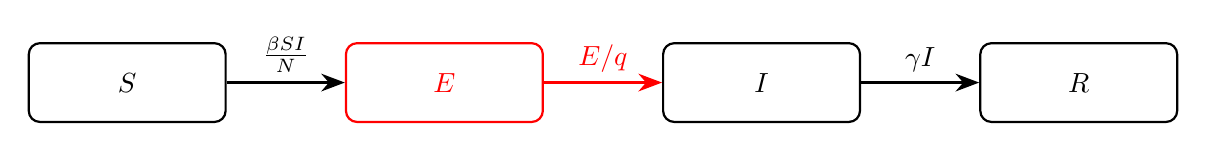
\begin{tikzpicture}[
		compartment/.style={
			rectangle,
			rounded corners,
			draw=black,
			thick,
			minimum width=2.5cm,
			minimum height=1cm,
			align=center
		},
		arrow/.style={
			thick,
			-{Stealth[length=3mm]},
		}
	]
	
	\node[compartment] (S) {$S$};
	\node[compartment, right=1.5cm of S, draw=red, text=red] (E) {$E$};
	\node[compartment, right=1.5cm of E] (I) {$I$};
	\node[compartment, right=1.5cm of I] (R) {$R$};
	
	\draw[arrow] (S) -- (E) node[midway, above] {$\frac{\beta S I}{N}$};
	\draw[arrow, red] (E) -- (I) node[midway, above] {$E / q$};
	\draw[arrow] (I) -- (R) node[midway, above] {$\gamma I$};
	
	\end{tikzpicture}

	{\bf ODEs:
	$$\dot{S} = \frac{-\beta S I}{N}$$
	\textcolor{red}{$$\dot{E} = \frac{\beta S I}{N} - \frac{E}{q}$$}
	$$\dot{I} = \frac{E}{q} - \gamma I$$
	$$\dot{R} = \gamma I$$
	}
	
	\item Suppose that we want to model Hospitalization, with the following assumption: Infected folks either recover directly {\it or} they are hospitalized first and then recover. Let the direct recovery rate be $\gamma$, and suppose that there are 4 direct recoveries for every 1 hospitalization. Let the typical duration of a hospitalization be $\delta$ days. Use the letter $h$ for the hospitalized compartment. Draw a flow diagram for the normalized system, and write a set of corresponding differential equations. You should assume that folks in the hospital do not come into contact with anyone else during their hospital stay.
	
	{\bf Flow diagram: }

	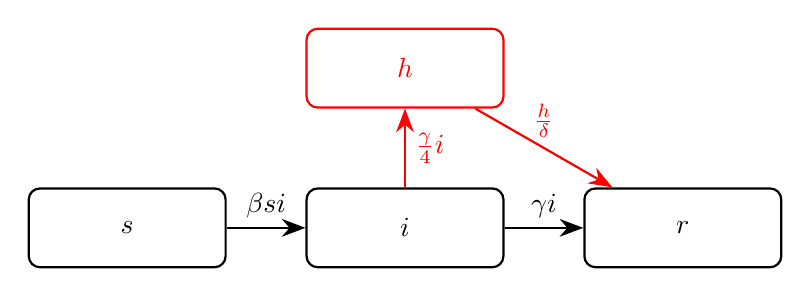
\begin{tikzpicture}[
		compartment/.style={
			rectangle,
			rounded corners,
			draw=black,
			thick,
			minimum width=2.5cm,
			minimum height=1cm,
			align=center
		},
		arrow/.style={
			thick,
			-{Stealth[length=3mm]},
		}
	]
	
	\node[compartment] (S) {$s$};
	\node[compartment, right=of S] (I) {$i$};
	\node[compartment, above=of I, draw=red, text=red] (H) {$h$};
	\node[compartment, right=of I] (R) {$r$};
	
	\draw[arrow] (S) -- (I) node[midway, above] {$\beta s i$};
	\draw[arrow] (I) -- (R) node[midway, above] {$\gamma i$};
	\draw[arrow, red] (I) -- (H) node[midway, right, red] {$\frac{\gamma}{4} i$};
	\draw[arrow, red] (H) -- (R) node[midway, above, red] {$\frac{h}{\delta}$};
	
	\end{tikzpicture}

	{\bf ODEs:
	$$\dot{s} = -\beta s i$$
	$$\dot{i} = \beta s i - \gamma i - \textcolor{red}{\frac{\gamma}{4} i}$$
	$$\textcolor{red}{\dot{h} = \frac{\gamma}{4} i - \frac{h}{\delta}}$$
	$$\dot{r} = \gamma i + \textcolor{red}{\frac{h}{\delta}}$$
	}
	
	\item Suppose that we want to model an infectious disease that afflicts a growing population of bacteria, such that the infection follows an SIR model, the bacteria grow according to a logistic growth model with intrinsic growth rate $\alpha$ and carrying capacity $K$. Let all bacteria reproduce, but suppose that susceptible and recovered bacteria produce susceptible progeny, while infected bacteria produce infected progeny. The carrying capacity is shared by all three bacteria. 

	{\bf The total bacteria population grows according to $$\dot{N} = \alpha N \left(1 - \frac{N}{K}\right),$$
	so the number of bacteria born into $S$ will be proportional to $(S + R) / N$ and the number born into $I$ will be proportional to $I / N$.}
	
	{\bf
	Flow diagram: }

	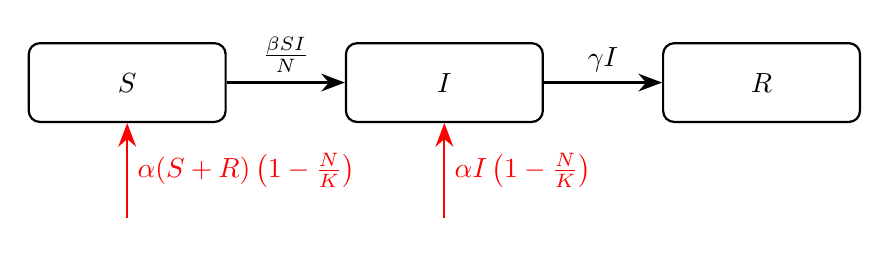
\begin{tikzpicture}[
		compartment/.style={
			rectangle,
			rounded corners,
			draw=black,
			thick,
			minimum width=2.5cm,
			minimum height=1cm,
			align=center
		},
		arrow/.style={
			thick,
			-{Stealth[length=3mm]},
		}
	]
	
	\node[compartment] (S) {$S$};
	\node[compartment, right=1.5cm of S] (I) {$I$};
	\node[compartment, right=1.5cm of I] (R) {$R$};
	
	\draw[arrow] (S) -- (I) node[midway, above] {$\frac{\beta S I}{N}$};
	\draw[arrow] (I) -- (R) node[midway, above] {$\gamma I$};

	\node[below=1.2cm of S] (birthS) {};
	\node[below=1.2cm of I] (birthI) {};

	\draw[arrow, red] (birthS) -- node[right] {$\alpha(S + R) \left(1 - \frac{N}{K}\right)$} (S);
	\draw[arrow, red] (birthI) -- node[right] {$\alpha I\left(1 - \frac{N}{K}\right)$} (I);
	
	\end{tikzpicture}

	{\bf ODEs:
	$$\dot{S} = -\frac{\beta S I}{N} + \textcolor{red}{\alpha (S + R) \left(1 - \frac{N}{K}\right)}$$
	$$\dot{I} = \frac{\beta S I}{N} - \gamma I + \textcolor{red}{\alpha I \left(1 - \frac{N}{K}\right)}$$
	$$\dot{R} = \gamma I$$
	}
\end{enumerate}

\end{enumerate}

\end{document}